\chapter{System Description}\label{chap:systemDescription}
The system is composed by a camera that captures the table that contains the bricks and a robot arm that is charge of picking and placing the brick to build the desired figures. The setup can be seen in \autoref{fig:setup}.
\begin{figure}[H]
    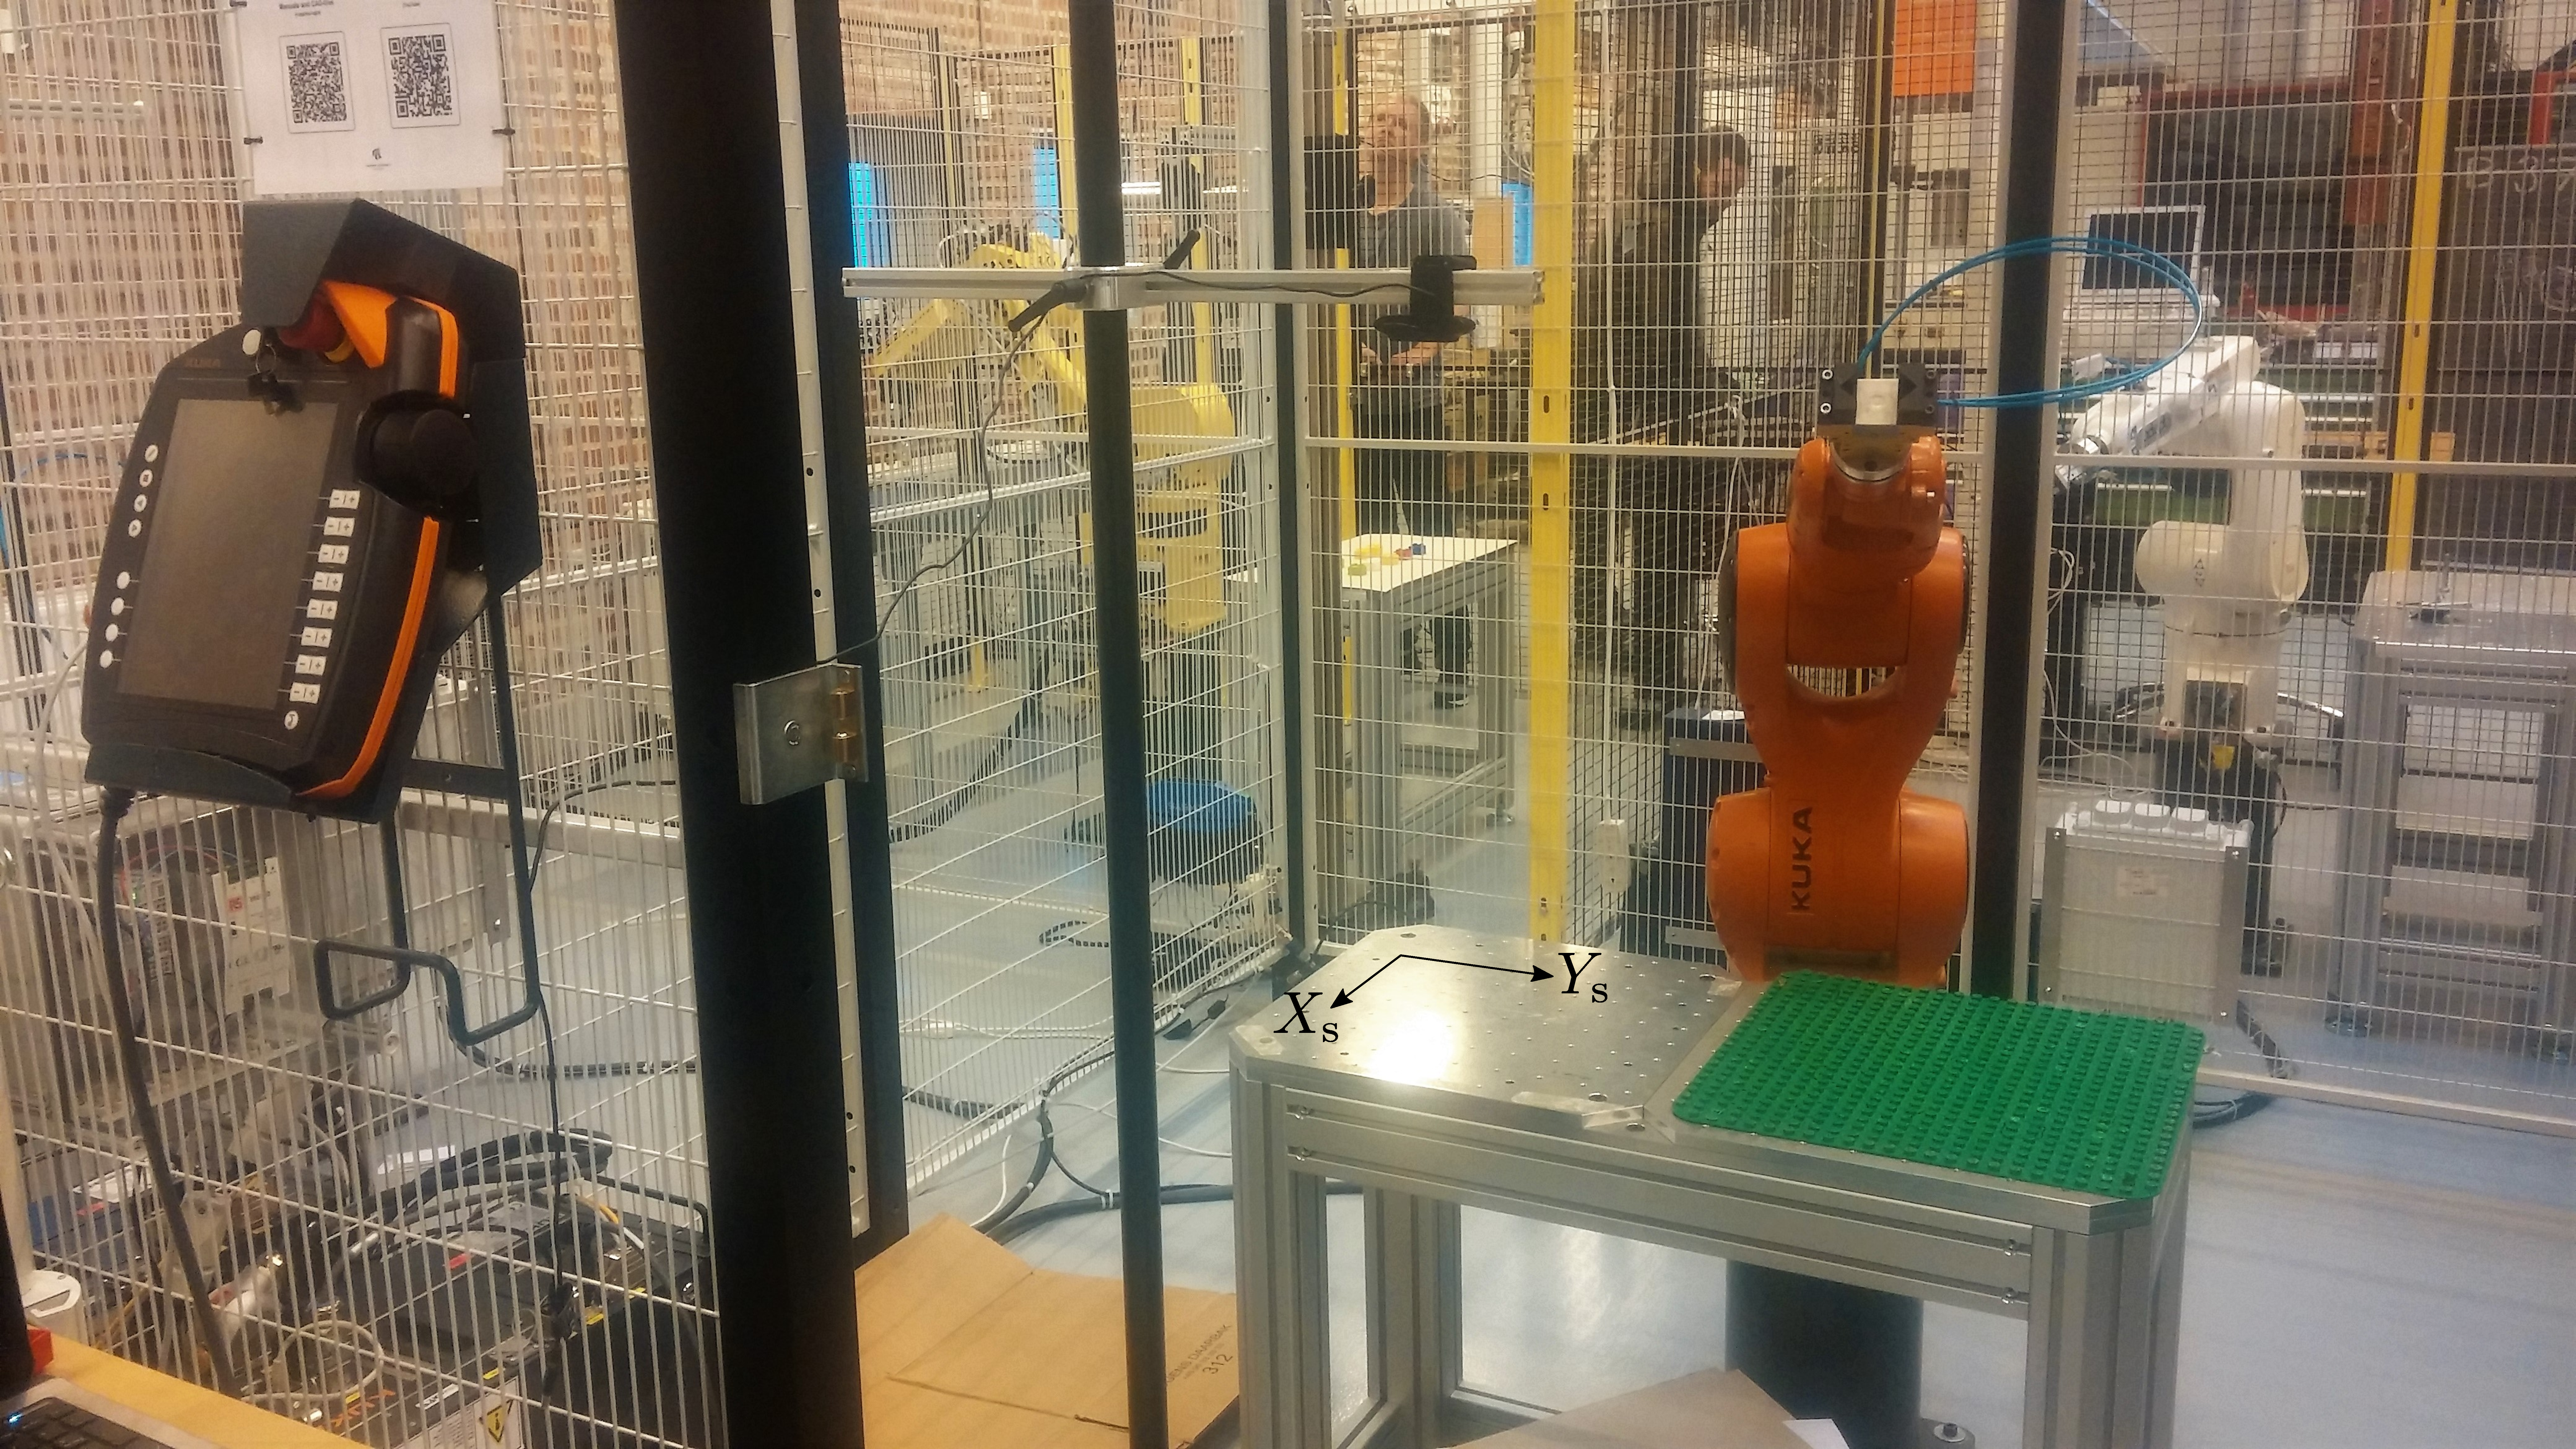
\includegraphics[width=0.5\textwidth]{figures/setup_axes.pdf}
    \caption{Image of the setup, where the robot cell can be seen. It contains the robot arm, the security fence, the camera and the table that is the base workspace of the system. }
    \label{fig:setup}
\end{figure}

The coordinate of the base workspace can be seen in \autoref{setup} and it is aligned with the robot's frame, but it starts at position (411.69,-285.27,340.12) in the robot's world frame, with respect to whom the coordinates need to be sent to the robot. Since all the positions are calculated with respect to the base frame, the offset is added before sending the command to the robot controller.
  
In this chapter more details about the robot arm and the camera are described. 

\section{Industrial Robot}
The industrial robot is a KUKA KR6 R700 and it is composed by a manipulator, a robot controller and a smartPAD teach pendant. 

The manipulator is a 6DOF robot arm that is made of six rotation joints. A diagram of the robot can be seen in \autoref{fig:kuka_axes}.
\begin{figure}[H]
    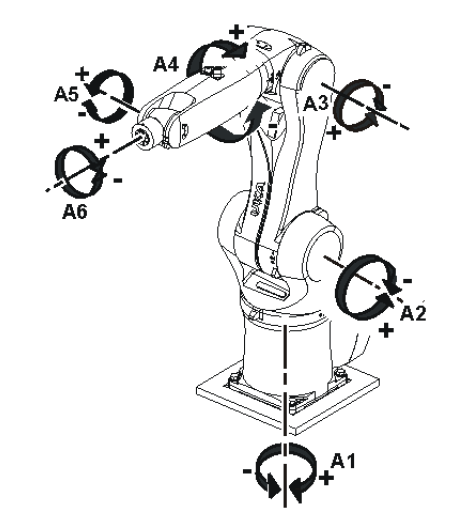
\includegraphics[width=0.25\textwidth]{figures/kuka_axes.png}
    \caption{.\cite{kuka} }
    \label{fig:kuka_axes}
\end{figure}

The interface with the robot controller is done through MATLAB. This provides an easier integration of the vision algorithms and the robot movement. A MATLAB class, \lstinline[style=matlabinline]{RobotConnectorKUKA.m}, connects to the robot controller and defines the functions needed to operate the manipulator. For this project the used functions can be seen in \autoref{MatlabFunctions}.

\begin{lstlisting}[ language = Matlab,
caption  = {Matlab functions used to operate KUKA robot.},
label    = MatlabFunctions ]
% Constructor of the class
obj = RobotConnectorKUKA(hostAddress_,hostPort_);
% Move to point with position (x,y,z) and orientation (w,p,r) in a linear motion
moveLinear(obj,x,y,z,w,p,r,speed);
% Open gripper
openGrapper(obj);
% CLose gripper
closeGrapper(obj);
\end{lstlisting}

In order to pick the bricks, a gripper needs to be designed based of the dimensions of the flange and the bricks. A drawing of the bottom view of the flange, where the gripper is attached can be seen in \autoref{fig:holder}, while the Lego brick dimensions can be seen in \autoref{fig:legobrick}.

\begin{figure}[H]
    \captionbox
    {
        Bottom view of the flange, where the gripper is attached.
        \label{fig:holder}                                 
    }                                                                 
    {                                                                  
        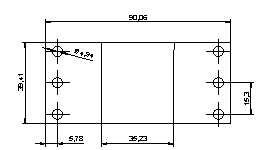
\includegraphics[width=.4\textwidth]{figures/holder}         
    }                                                                   
    \hspace{5pt}
    \captionbox
    {
        Diagram of a Lego piece.
        \label{fig:legobrick}                                     
    }                                                                           
    {                                                                            
        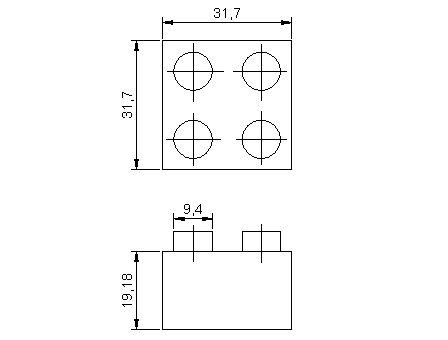
\includegraphics[width=.4\textwidth]{figures/LegoPiece}            
    }                                                                            
\end{figure}
The design of the gripper is done such that when it is open it has enough space to grab the piece while being able to lead it to the right orientation when it is closed, and it is also able to push the brick in the final position. These features ease the pick and place operations. A drawing of the final design of the gripper can be seen in \autoref{fig:gripper}.

\begin{figure}[H]
    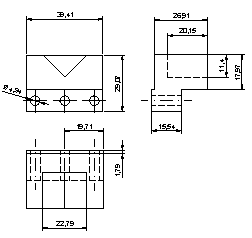
\includegraphics[width=.4\textwidth]{figures/gripper}
    \caption{Diagram of the gripper that includes the dimensions.}
    \label{fig:gripper}  
\end{figure}


\section{Camera} \label{sec:camera}
The position and orientation of the blocks are obtained from images taken with Logitech HD Pro Webcam C920. This device can be seen in \autoref{fig:camera}.
\begin{figure}[H]
    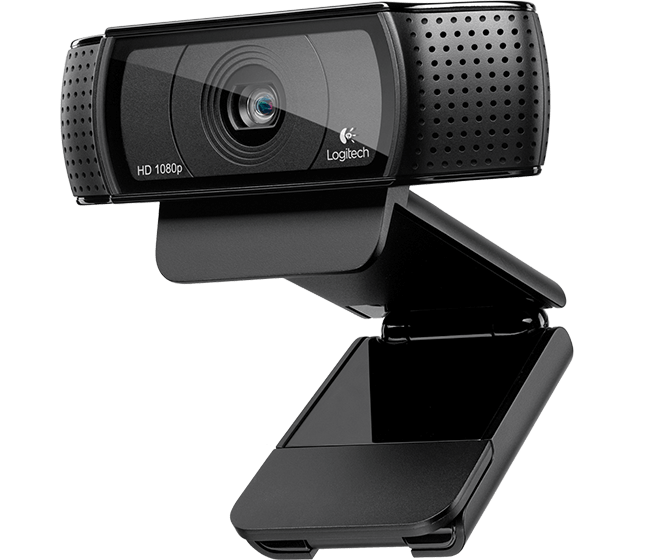
\includegraphics[width=0.2\textwidth]{figures/camera.png}
    \caption{Logitech HD Pro Webcam C920 used to locate the Lego bricks.\cite{camera} }
    \label{fig:camera}
\end{figure}
The camera has been placed in the robot cell as in \autoref{fig:setup}. In order to use the images, a projection matrix that translates the image points into scene points needs to be found. As all desired goals lay on the same plane, the projection matrix can be found using pairs of points that have correspondence in the scene and in the image.

\autoref{fig:points} shows the points used in the scene, in this case the threaded holes in the table which are 40 mm apart. The black axes define the base coordinate frame and the red dots are the ones used in the projection matrix calculation.
\begin{figure}[H]
	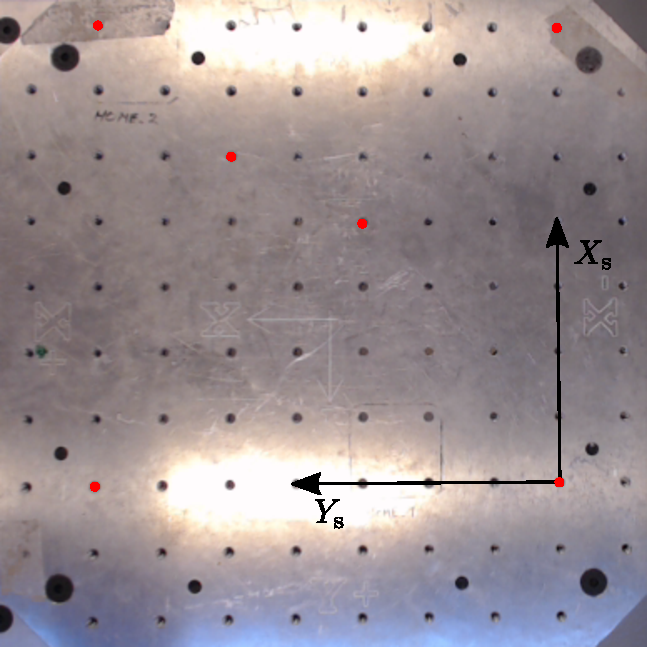
\includegraphics[width=0.25\textwidth]{figures/dots_cut.pdf}
	\caption{Image used to find the projection matrix. The black axes define the base coordinate frame and the red dots are the ones used in the projection matrix calculation. }
	\label{fig:points}
\end{figure}
The projection matrix found is
\begin{flalign}
    \vec{H}=
    \begin{bmatrix}
        -0.0086 & -1.0150 & 296.0846 \\
        -1.0165 & 0.0028 & 340.7488 \\
        0 & 0 & 1 
    \end{bmatrix} \label{eq:projectionmatrix}
\end{flalign}
With this matrix any image point given in pixel coordinates can be translated into scene coordinates.
